\documentclass{article}

\usepackage{fancyhdr}
\usepackage{extramarks}
\usepackage{amsmath}
\usepackage{amsthm}
\usepackage{amssymb}
\usepackage{amsfonts}
\usepackage{tikz}
\usepackage[plain]{algorithm}
\usepackage{algpseudocode}
\usepackage{nameref}
\usepackage{cite}
\usepackage{tikz-cd}
\usepackage{mathrsfs}
\usepackage{tikz}
\newcommand*\circled[1]{\tikz[baseline=(char.base)]{
            \node[shape=circle,draw,inner sep=2pt] (char) {#1};}}

\usetikzlibrary{automata,positioning}


\topmargin=-0.45in
\evensidemargin=0in
\oddsidemargin=0in
\textwidth=6.5in
\textheight=9.0in
\headsep=0.25in

\linespread{1.1}

\pagestyle{fancy}
\chead{\hmwkTitle}
\lhead{\hmwkAuthorName}
\rhead{\hmwkClass}
\cfoot{\thepage}

\renewcommand\headrulewidth{0.4pt}
\renewcommand\footrulewidth{0.4pt}
\newcommand{\sur}[1]{\ensuremath{^{\textrm{#1}}}}
\newcommand{\sous}[1]{\ensuremath{_{\textrm{#1}}}}
\newcommand{\Hom}{\text{Hom}}
\newcommand{\Tor}{\text{Tor}}
\newcommand{\Ext}{\text{Ext}}
\newcommand{\bb}[1]{\mathbb{#1}}
\newcommand{\fk}[1]{\mathfrak{#1}}
\newcommand{\iso}{\cong}
\newcommand{\del}{\partial}

\setlength\parindent{0pt}

%c
% Create Problem Sections
%

\newtheorem{lemma}{Lemma}
\newtheorem{exercise}{Exercise}
%
% Homework Details
%   - Title
%   - Due date
%   - Class
%   - Section/Time
%   - Instructor
%   - Author
%

\newcommand{\hmwkTitle}{Homework 2}
\newcommand{\hmwkDueDate}{Oct 18th, 2019}
\newcommand{\hmwkClass}{Math 246A Complex Analysis}
\newcommand{\hmwkClassInstructor}{Professor Rowan Killip}
\newcommand{\hmwkAuthorName}{\textbf{Anish Chedalavada}\\ Collaborators: Nicholas Liskij}

%
% Title Page
%

\title{
    \vspace{2in}
    \textmd{\textbf{\hmwkClass:\ \hmwkTitle}}\\
    \vspace{0.1in}
    \textmd{\hmwkDueDate} \\
    \vspace{0.2in}\large{\textit{\hmwkClassInstructor\  }}
    \vspace{2in}
}

\author{\hmwkAuthorName}

\date{}

\begin{document}
\maketitle
\newpage

\begin{exercise}
  a) Let $\Omega \in \bb{C}$ be open. Suppose $f: \Omega \to \bb{C}$ is smooth; show that
  \[
    \Delta f = 4 \partial_{z}\partial_{\bar{z}}f
  \]
  b) Let $f: \Omega \to \bb{C}$ and distributionally holomorphic. Show that $f$ is distributionally harmonic. \\
  c) Show the a smooth function $f:\Omega \to \bb{C}$ is harmonic if and only if it is distributionally harmonic.
\end{exercise}

\begin{proof}
  a) We have that $\partial_{x} = \partial_{z} + \partial_{\bar{z}}, \ \partial_{y} = i(\partial_{z} - \partial_{\bar{z}})$, and so $\partial_{x}^{2} + \partial_{y}^{2} = (\partial_{z} + \partial_{\bar{z}})^{2} - (\partial_{z} - \partial_{\bar{z}})^{2} = 4 \partial_{z}\partial_{\bar{z}}$. \\
  
  b) Consider the integral:
  \[
    \int\limits_{\bb{C}}f(x+iy)[\Delta\phi](x+iy) \ dx \ dy = \int\limits_{\bb{C}}f(x+iy)[4 \partial_{z}\partial_{\bar{z}}\phi](x+iy) \ dx \ dy = 4 \int\limits_{\bb{C}}f(x+iy)[\partial_{\bar{z}}\partial_{z}\phi](x+iy) \ dx \ dy = 0  
  \]
  Where the step $\del_{z}\del_{\bar{z}} = \del_{\bar{z}}\del_{z}$ comes from expanding out the formulas and using Clairaut's Theorem on $\del_{x}, \ \del_{y}$, and the last equality comes from $f$ being distributionally holomorphic. \\
    
  c) Suppose $f$ is distributionally harmonic. Let $\phi$ be an arbitrary smooth function of support properly contained in some compact set $K$. We may thus evaluate the integral
  \[
    \int\limits_{\bb{C}}f(x+iy)[\Delta\phi](x+iy) \ dx \ dy = \int\limits_{K}f(x+iy)[\Delta\phi](x+iy) \ dx \ dy
  \]
  As the function has support properly contained in $K$ and thus the integral is zero outside $K$.
  For $f$ smooth we may apply the formula for integration by parts:
  \[
    \int\limits_{K}f(x+iy)[4\del_{z}\del_{\bar{z}}\phi](x+iy) \ dx \ dy = \int\limits_{K}\phi(x+iy)[4\del_{z}\del_{\bar{z}} f](x+iy) \ dx \ dy = \int\limits_{\bb{C}}\phi(x+iy)[4\del_{z}\del_{\bar{z}} f](x+iy) \ dx \ dy = 0
  \]

  Where all products $\phi \cdot f$ in the expansion disappear on the boundaries of $K$ (as support lies inside $K$), and the last equality comes from $f$ being distributionally harmonic. As $\phi$ was an arbitrary function of compact support, we have that the integral $\int\limits_{\bb{C}}\phi(x+iy)[4\del_{z}\del_{\bar{z}} f](x+iy) \ dx \ dy$ disappears for every smooth function $\phi$ of compact support. As $[4\del_{z}\del_{\bar{z}} f](x+iy)$ is smooth, this implies it is $0$ and thus $f$ is harmonic. Conversely, supposing $f$ is harmonic, for any arbitrary function $\phi$ of compact support we may apply the same integration by parts process to change the integral to
  \[
    \int\limits_{\bb{C}}\phi(x+iy)[4\del_{z}\del_{\bar{z}} f](x+iy) \ dx \ dy = 0
  \]
  As $[4\del_{z}\del_{\bar{z}} f](x+iy) = 0$ by assumption, and thus $f$ is distributionally harmonic. 
\end{proof}

\begin{exercise}
  a) Prove Green's Theorem: i.e., given a triangle with vertices $0, \ a, \ ib$, $a,b > 0$, and a $C^{1}$ function $f: \bb{C} \to \bb{C}$, we have that:
  \[
    2i \iint_{T} [\del_{\bar{z}}f](x+iy) \ dx \ dy = \int_{\del T}f(z) dz 
  \]
  b) Extend part a) to all triangles. \\
  c) + d) Show Goursat's Theorem for everywhere holomorphic functions using the previous result and justify your assumptions on the domain of $f$ and $\del_{\bar{z}} f$ \\
  e) Exhibit an example of a smooth function that satisfies $\del_{\bar{z}} f(z) = 0$ for $\frac{1}{2} < |z| < 2$ but for which the line integral around the unit circle does not vanish.
\end{exercise}
\begin{proof}
  a) Let $\gamma$ denote the straight line from $a$ to $ib$, oriented from $a$ to $ib$. Consider the following string of derivations:
  \newpage
  \begin{align*}
    & 2i \iint_{T} [\del_{\bar{z}}f](x+iy) \ dx \ dy = \iint_{T} [(i\del_{x} - \del_{y})f](x+iy) \ dx \ dy \\
    = \ & \iint_{T} [i\del_{x}f](x+iy) \ dx \ dy   - \iint_{T} [\del_{y}f](x+iy) \ dx \ dy \\
    = \ & \int_{0}^{a}\int_{0}^{\frac{-b}{a}x + b}[i\del_{x}f](x+iy) \ dy \ dx - \int_{0}^{a}\int_{0}^{\frac{a}{b} + a}[\del_{y}f](x+iy) \ dx \ dy \\
    = \ & \int\limits_{0}^{ib}if(y \frac{a}{b} + a + iy) - if(iy) \ dy - \int\limits_{0}^{a}f(i(x \frac{-b}{a} + b) + x) + f(x) \ dx \text{ --- } \circled{1}\\
    \rightarrow \ & \int\limits_{0}^{ib}if(y \frac{a}{b} + a + iy)dy  = i \int\limits_{\gamma}f(x+iy)dy, \ \int\limits_{a}^{0} f(i(x \frac{-b}{a} + b) + x)dx =  \int\limits_{\gamma}f(x+iy)dx \\
    \implies  \ &\circled{1} = - i\int\limits_{0}^{ib}f(iy) \ dy + \int\limits_{0}^{a}f(x) dx  \int\limits_{\gamma}f(x+iy) dx + \int\limits_{\gamma}if(x+iy)dy \\
    = \ & \int\limits_{\gamma_{1}}f(z)dz + \int\limits_{\gamma_{2}}f(z)dz + \int\limits_{\gamma_{3}}f(z)dz = \int\limits_{\del T}f(z) d(z)
  \end{align*}
  Where $\gamma_{1}$ is the line from $ib$ to 0, $\gamma_{2}$ is the line from 0 to $a$, and $\gamma_{3} = \gamma$ the line from $a$ to $ib$: it is clear that these orientations are reflected in the second to last line above. \\

  b) It suffices to check the claim on right angled triangles, as any triangle may be bisected into right angled triangles by dropping a perpendicular from any vertex and thus the integral over the whole triangle is the sum of integrals over each right angled triangle. Given a right angled triangle $T$ in the complex plane we may apply a translation and a rotation to have a triangle of the form in $a)$, namely with one side on the imaginary and one side on the real axes. Thus, we write $g = f(w_{0} + e^{i\theta_{0}}z)$ to denote precomposing with this translation and rotation, such that $g$ satisfies the claim from $a)$ over the translated triangle $T'$ and thus $f$ satisfies it over the triangle $T$. \\

  c) + d) For any rectifiable curve we have the diagram below given some polygonal approximation to it; indicating that we may write the integral over this polygonal approximation as the sum of integrals over triangles with base some line segment and fixed vertex enclosed by $\gamma$. We have that the integral over any triangle is given by Green's Theorem above, i.e. that $\int\limits_{\del T}f(z)dz = \iint_{T}[\del_{\bar{z}}f](x+iy)dxdy$. Note that we utilise the assumption that $f$ and $\del_{\bar{z}} f$ are defined over the region enclosed by any triangle corresponding to this polygonal approximation in order to take the integral over the region. Given that $\gamma$ is arbitrary enclosing any point in $\bb{C}$, this requires that $f$ and $\del_{\bar{z}}$ be defined over all of $\bb{C}$. As $\del_{\bar{z}}f$ is identically zero throughout the complex plane, we have that $\int\limits_{\del T}f(z)d(z)$ must also be zero for any triangle in the complex plane. Thus, for any polygonal approximation to a rectifiable curve $\gamma$, the integral over the polygonal path must also be $0$ as it is the sum of integrals over triangles. As the integral over a rectifiable curve is the supremum of the integral over all its polygonal approximation, we have that the integral over the curve $\gamma$ must be $0$.
  
  \begin{center}
    
\tikzset{every picture/.style={line width=0.75pt}} %set default line width to 0.75pt        

\begin{tikzpicture}[x=0.75pt,y=0.75pt,yscale=-1,xscale=1]
%uncomment if require: \path (0,300); %set diagram left start at 0, and has height of 300

%Shape: Polygon Curved [id:ds567845403603723] 
\draw   (260.88,38.31) .. controls (293.17,22.96) and (436.86,4.54) .. (427.18,64.4) .. controls (417.49,124.26) and (545.04,168.77) .. (457.85,237.85) .. controls (370.67,306.92) and (285.1,273.15) .. (243.92,190.26) .. controls (202.75,107.38) and (228.59,53.66) .. (260.88,38.31) -- cycle ;
%Shape: Triangle [id:dp4719139952177067] 
\draw   (343.81,134.56) -- (225.1,126.03) -- (239.79,57.58) -- cycle ;
%Shape: Triangle [id:dp20711645759682185] 
\draw   (343.34,134.71) -- (239.92,57.82) -- (296.5,27) -- cycle ;
%Straight Lines [id:da40834350062676306] 
\draw    (383.5,27) -- (343.81,134.56) ;


%Straight Lines [id:da5836908416711326] 
\draw    (383.03,27.14) -- (296.5,27) ;


%Straight Lines [id:da08423742981304261] 
\draw    (225.1,126.03) -- (256.5,214) ;


%Straight Lines [id:da8011966326487425] 
\draw    (343.34,134.71) -- (256.5,214) ;


%Curve Lines [id:da5894318426258609] 
\draw    (332.5,194) .. controls (384.24,250.72) and (464.69,181.7) .. (413.28,139.63) ;
\draw [shift={(412.5,139)}, rotate = 398.4] [color={rgb, 255:red, 0; green, 0; blue, 0 }  ][line width=0.75]    (10.93,-3.29) .. controls (6.95,-1.4) and (3.31,-0.3) .. (0,0) .. controls (3.31,0.3) and (6.95,1.4) .. (10.93,3.29)   ;


% Text Node
\draw (382,12) node  [align=left] {a};
% Text Node
\draw (235,221) node  [align=left] {b};


\end{tikzpicture}
\end{center}

e) Consider the indicator function $\chi_{>\frac{1}{4}}$ that is 1 on the complex plane outside of the disk of radius $\frac{1}{4}$ and $0$ inside. Consider the convolution $\phi = \chi_{{> 1/4 }} * \psi_{\epsilon}$ for $\psi_{\epsilon}$ a mollifier with $\epsilon < \frac{1}{8}$. We have that $\phi(z)$ is smooth, 1 outside the disk of radius $1/4$, and $0$ on some sufficiently small disk containing the origin. Furthermore, we have that the function $g(z) = \phi(z)\cdot 1/z$ is smooth everywhere excluding the origin, and may be smoothly extended to $g(0) = 0$ as it is identically zero on a neighborhood of the origin. Thus, we have a smooth function such that in the annulus $\frac{1}{2}< |z| < 2$ it satisfies the relations $\del_{\bar{z}}g \equiv 0$ as in this annulus it is equal to the function $1/z$, which is holomorphic everywhere except the origin. However, consider the following integral:
\[
  \int\limits_{S^{1}} g(z)d(z) = \int\limits_{S^{1}}\frac{1}{z} = 2 \pi i \cdot 1
\]
Via the Cauchy Integral formula expansion for the constant function $z \mapsto 1$. 
\end{proof}

\begin{exercise}
  Let $\Omega \subset \bb{C}$ be open and $f_{n}: \Omega \to \bb{C}$ be holomorphic. Suppose that for each compact set $K \subset \Omega$ the functions $f_{n}$ converge uniformly to some $f: \Omega \to \bb{C}$. Show that $f$ must itself be holomorphic.  
\end{exercise}
\begin{proof}
We first show that the $f_{n}'$ converge uniformly. For any connected compact set $K \subset \Omega$ with boundary a closed curve $\gamma$, and length$(\gamma) = l$. Let $k \subset K$ be the compact subset of elements that are of distance at least $\xi > 0$ from the boundary of $K$. Fix $\epsilon > 0$. For any $w \in k$, we may select $N \in \bb{N}$ s.t. for $m,n > N$, $|f_{m}(w) - f_{n}(w)| < \frac{\epsilon \xi^{2}}{l}$. Using this in conjuction with the Cauchy integral formula for the derivative, we have:
  \[
    |f'_{n}(w) - f'_{m}(w)| \leq \int\limits_{0} \frac{|f_{m}(\gamma(t)) - f_{n}(\gamma(t))|}{|\gamma(t)-w|^{2}}  |\gamma'(t)| dt\leq \int\limits_{\gamma} \frac{|f_{m}(\gamma(t)) - f_{n}(\gamma(t))|}{\xi^{2}} dt \leq \frac{\epsilon \xi^{2}}{l}\cdot \frac{l}{\xi^{2}}
  \]
  And thus $|f'_{n}(w) - f'_{m}(w)| < \epsilon$ for $n,m > N$, implying they converge uniformly on $k$. Note that as $\Omega$ is open, any connected compact set $k$ is properly contained in the interior of a larger compact set $K$, yielding that every element of $k$ is a positive distance from the boundary of $K$, and this admits a minimum. Thus, the convergence condition on arbitrary compact sets for $f_{n}$ yields uniform convergence on arbitrary compact sets in $\Omega$ for $f_{n}'$. Thus, the $f_{n}'(z)$ converge uniformly to some limit $g(z)$. Now we shall show that for any path $\gamma$ from $z_{0}$ to $z$, the function $G(\zeta) = \int\limits_{\gamma}g(\zeta)d\zeta$ is well defined (i.e. independent of path from $z_{0}$ to $z$) and holomorphic with derivative $g(\zeta)$. We have that for any path $\gamma$, $\int\limits_{\gamma}g(\zeta)d\zeta = lim_{n\to \infty}\int\limits_{\gamma}f_{n}'(\zeta)d\zeta$ by uniform convergence on compact sets, and we note that the integrals on the right are independent of path $\gamma$: given distinct paths $\gamma_{1}$, $\gamma_{2}$ from $z_{0}$ to $z$ this can be seen as
  \[
    \int\limits_{\gamma_{1}}f_{n}'(\zeta)d\zeta - \int\limits_{\gamma_{2}}f_{n}'(\zeta)d\zeta = \int\limits_{\gamma_{1}-\gamma_{2}}f_{n}'(\zeta)d\zeta = 0
  \]
  Due to the Cauchy-Gorsat theorem for holomorphic functions. Thus, the limit must be the same regardless of the path $\gamma$ from $z$ to $z_{0}$, and thus the value of $\int\limits_{\gamma}g(\zeta)d\zeta$ is independent of path. We may thus omit the $\gamma$ from the notation and write the integral with the limits $z_{0}, z$. Fix $\epsilon>0$, let $\Delta \in \bb{C}$ with $\Delta + z \in \Omega$, and $|z - w| < |\Delta| \implies |f(z) - f(w)| < \epsilon$. Consider the following sequence of derivations:
  \begin{align*}
    \left| \frac{G(z + \Delta) - G(z)}{\Delta} - g(z) \right | \leq  \ \frac{1}{|\Delta|}\left|\int\limits_{z}^{z+\Delta}f(\zeta) d\zeta - \Delta f(z) \right | = \frac{1}{|\Delta|}\left|\int\limits_{z}^{z+\Delta}f(\zeta) - f(z)d\zeta \right| \\
    \leq \  \frac{1}{|\Delta|}\int\limits_{z}^{z+\Delta}|f(\zeta)-f(z)| |d\zeta| \leq \frac{1}{|\Delta|}\epsilon|\Delta| = \epsilon
  \end{align*}
  For all $\epsilon > 0$ we may select $\Delta$ small enough such that the difference on the left is less than $\epsilon$, implying the limit as $\Delta \to 0$ must be $0$. Thus, the derivative for $G$ exists at $z$ and is $g(z)$. Let $z_{0}\in \bb{C}$ fixed and $z \in \bb{C}$ arbitrary, with $\gamma$ a path from $z_{0}$ to $z$:
  \[
    \int\limits_{\gamma}f'_{n}(\zeta)d\zeta = \int\limits_{0}^{1}f_{n}'(\gamma(t))\cdot\gamma'(t)dt = \int\limits_{0}^{1}\frac{d}{dt}(f_{n}(\gamma(t)))dt = f_{n}(z) - f_{n}(z_{0})
  \]
  As $n \to \infty$, we have that the limit must agree with the limit on the right and so we have:
  \[
    \int\limits_{\gamma}g(\zeta)d\zeta = f(z) - f(z_{0}) \implies \int\limits_{\gamma}g(\zeta)d\zeta +f(z_{0}) = f(z) 
  \]
  And we know from above that $\int\limits_{\gamma}g(\zeta)d\zeta +f(z_{0})$ is independent of path and holomorphic in $z$. Thus, $f(z)$ is holomorphic in $z$, and we know from above that $f'(z) = g(z)$, implying that $f'_{n}$ converge uniformly to $f'$
\end{proof}


The following lemma is used for the later exercises: \\

\underline{\bf Lemma} \textit{Let $f$ be a holomorphic function in a connected region $\Omega \subset \bb{C}$ admitting a limit point of zeroes. Then f $\equiv 0$ in $\Omega$}.
\begin{proof}
   Let $f($ $z_{n} \in \Omega \cap f^{-1}(0)$ be a sequence of zeroes converging to a limit point $z$. W.l.o.g. we may assume $z=0$ by instead considering the function $h:w \mapsto f(w+z)$. Relabel $f=h$. By analyticity, we have that in a neighborhood $0 \in N$, $f$ has a power series expansion with no constant term (as it is 0 at 0). Thus, we have that $f_{1} = \frac{f(w)}{w}$ is also analytic in $N$. We have that arbitrarily close to $0$, we may select points $z_{n} \in N$ convering to $0$ s.t. $f(z_{n}) = 0$ and thus $f_{1} = \frac{f(z_{n})}{z_{n}} = 0$, and by continuity this implies $f_{1}(0) = 0$. This yields that the constant term for $f_{1}$ is $0$. Continuing this process recursively, we obtain that for the expansion $f(z) = \sum_{k=0}^{\infty}a_{k}z^{k}$ that all terms $a_{k}$ must be $0$ by repeatedly dividing by $z$ and showing that the coefficient of $z^{1}$ is $0$. Thus, $f$ is identically $0$ in a nieghborhood of $0$. We thus have that the set of limit points of sequences in $f^{-1}(0) \cap \Omega$ is a closed subset of $\Omega$ in the subspace topology, being a closed subset of $f^{-1}(0)$ which is itself closed. However, it is also an open subset of $\Omega$ as every limit point in $f^{-1}(0)$ has a neighborhood around it on which $f$ is identically $0$, which must be contained in the set of limit points. Thus, it is a clopen subset of $\Omega$, implying it is all of $\Omega$ by connectedness. Thus, $\Omega \subset f^{-1}(0)$, yielding the required claim.
\end{proof}
\newpage 
\begin{exercise}
  a) Prove Louiville's Theorem: Suppose $f: \bb{C}\to \bb{C}$ is holomorphic and
  \[
    |f(z)| \leq C(1+ |z|)^{n}
  \]
  for some $C>0$ and integer $n \geq 0$, then $f$ is a polynomial of degree not exceeding $n$. \\
  b) Suppose $g$ is holomorphic on $\Omega \setminus \{0\}$ for $\Omega$ a neighborhood of $0$ such that:
  \[
    |g(z)| \leq C|z|^{-n}
  \]
  Show that there is a holomorphic $h: \Omega \to \bb{C}$ and coefficients $a_{1},...,a_{n} \in \bb{C}$ so that
  \[
    g(z) = h(z) + \sum_{k=1}^{n} a_{k}z^{-n}
    \]
\end{exercise}
\begin{proof}
  a) We prove the base case first: Suppose we have that $|f(z)| \leq C$ for some constant $C$. Let $w \in \bb{C}$ arbitrary. We have Cauchy's integral formula for the $n+1$th derivative at $f(w)$, given by the series expansion:
  \[
    f^{(n+1)}(w) = \frac{n+1!}{2\pi i} \int\limits_{\gamma} \frac{f(z)}{(z-w)^{n+2}} \ dz
  \]
  Let $\gamma$ be a circle of arbitrary radius $r$ around the point $w$. Consider the following sequence of derivations:
  \begin{align*}
    f^{(n+1)}(w) = \frac{n+1!}{2\pi i} \int\limits_{\gamma} \frac{f(z)}{(z-w)^{n+2}} \ dz \implies  \ & |f^{(n+1)}(w)| \leq  \frac{n+1!}{2\pi } \int\limits_{0}^{1} \frac{|f(\gamma(t))|}{r^{n+2}} \cdot |\gamma'(t)| dt \\ 
  \end{align*}

  Note that the condition $|f(z)| \leq C(1 + |z|^{n})$ implies the maximum of $|f(z)|$ subject to the constraint $\gamma$ is less than or equal to $C(1 + (|w|+r)^{n})$, $|w| + r$ being the distance of the furthest point from the origin on the circle. Noting this, we have:
  \[
    \implies \ |f^{(n+1)}(w)| \leq \frac{n+1!}{2 \pi} C[1 + (|w|+r)^{n}] \cdot \frac{2\pi r}{r^{n+2}} = (n+1! C) \cdot \frac{1 + (|w| + r)^{n}}{r^{n+1}}
  \]
  We may pick arbitrary circles of radius $r$ which satisfy the above inquality. As $r \to \infty$ the numerator on the right grows $O(r^{n})$ while the denominator grows $O(r^{n+1})$. Thus, as $r \to \infty$ the quantity on the right goes to $0$, yielding that $|f^{n+1}(w)| < \epsilon$ for any $\epsilon > 0$, given that we may select $r$ such that the quantity on the right is less than $\epsilon$. Thus, $|f^{(n+1)}(w)| = 0$, and as $w \in \bb{C}$ was arbitrary we have that $f^{n+1}$ is uniformly zero. As holomorphic functions are analytic in every neighborhood with coefficients $\frac{f^{k}}{k+1!}$ we have that in every neighborhood they are a polynomial of degree not greater than $n$ (as the $n+1$th term onwards is always $0$). Let $N$ be an arbitrary neighborhood in $\bb{C}$ with associated polynomial expansion $p_{N}$ (of not more than degree $n$. We have that $p_{N}-f$ is holomorphic in $\bb{C}$ and thus the set $(p_{N}-f)^{-1}(0)$ is open and thus admits a limit point. This implies that $p_{N} - f \equiv 0$ in $\bb{C}$ and so $f = p_{N}$. \\

  b) We prove the base case first, for $g$ as above and $n = 0$. Let $\gamma$ be a contour given by the boundary of some disk $D$ of radius $r$ centered at the origin, such that $D \setminus \{0\}$ is contained in $\Omega$. Define the function $h$ by:
  \[
    h(w) = \frac{1}{2\pi i}\int\limits_{\gamma} \frac{g(z)}{z-w}
  \]
  \newpage
  The above is well defined at every point $v \notin \gamma$. Let $w \in \bb{C}$ arbitrary. Fix an $\epsilon> 0$. For  $0 < \delta < \epsilon\left|\frac{\min \ |z-w|^{2}}{\max \ g(z)|_{\gamma}}\cdot\frac{1}{r}\right| $, we have for $h \in \bb{C}$ with $|h| < \delta$, the following string of manipulations:
  \begin{align*}
    & \frac{1}{2 \pi}\left| \ \int\limits_{\gamma} \frac{g(z)}{z-w}dz - \int\limits_{\gamma} \frac{g(z)}{z-w + h}dz \ \right| \leq \ \frac{1}{2\pi} \ \int\limits_{0}^{1} \frac{|hg(\gamma(t))|}{|(\gamma(t)-w)^{2} + (\gamma(t)-w)h|}\cdot |\gamma'(t)| dt \\
    \leq \ & \frac{1}{2 \pi}\int\limits_{0}^{1} \frac{\delta |g(\gamma(t))|}{|(\gamma(t)-w)^{2}|} \cdot |\gamma'(t)|dt \leq \delta \left|\frac{\max \ g(z)|_{\gamma}}{\min \ |z-w|^{2}}\right|\frac{1}{2\pi} \cdot 2 \pi r \leq \epsilon
  \end{align*}
  And so $h$ is continuous at every point not in $\gamma$. Now consider the following diagram of $D$:

\begin{center}
\tikzset{every picture/.style={line width=0.75pt}} %set default line width to 0.75pt        
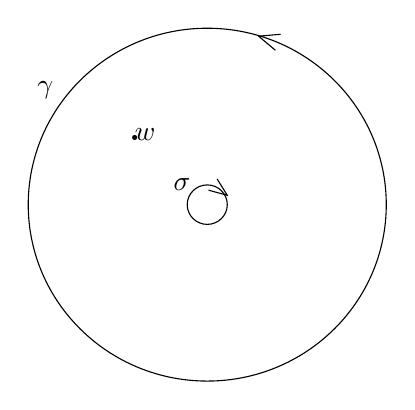
\begin{tikzpicture}[x=0.75pt,y=0.75pt,yscale=-1,xscale=1]
%uncomment if require: \path (0,300); %set diagram left start at 0, and has height of 300

%Shape: Ellipse [id:dp5122058783910688] 
\draw   (188,112) .. controls (188,65.06) and (226.62,27) .. (274.25,27) .. controls (321.88,27) and (360.5,65.06) .. (360.5,112) .. controls (360.5,158.94) and (321.88,197) .. (274.25,197) .. controls (226.62,197) and (188,158.94) .. (188,112) -- cycle ;
%Shape: Ellipse [id:dp8341447594648694] 
\draw   (264.6,112) .. controls (264.6,106.75) and (268.92,102.49) .. (274.25,102.49) .. controls (279.58,102.49) and (283.9,106.75) .. (283.9,112) .. controls (283.9,117.25) and (279.58,121.51) .. (274.25,121.51) .. controls (268.92,121.51) and (264.6,117.25) .. (264.6,112) -- cycle ;
\draw   (307.1,37.64) -- (299.01,30.83) -- (309.61,29.92) ;
\draw   (279.01,99.63) -- (283.89,107.49) -- (274.88,105.03) ;

% Text Node
\draw (262.06,102.49) node  [align=left] {$\displaystyle \sigma $};
% Text Node
\draw (196.23,56.94) node  [align=left] {$\displaystyle \gamma $};
% Text Node
\draw (239.28,80.03) node [scale=1.7280000000000002] [align=left] {.};
% Text Node
\draw (244.34,78.16) node  [align=left] {$\displaystyle w$};


\end{tikzpicture}

\end{center}

Fix $\epsilon >0$. Let $w\in D\setminus \{0\}$. Let $0< a < |w|$ for $a \in \bb{R}$ some fixed value. Let $\sigma$ be an circle around the origin oriented negatively to $\gamma$ of radius $k \leq \min(\frac{|w|}{4}, \epsilon \frac{|w| -a}{C})$. We have the annulus form of the Cauchy integral formula, given by (this is seen by dividing the annulus into two and noting that one contains $w$ and the other does not, implying the one containing $w$ yields $g(w)$ by the regular formula while the other is 0):
\[
  g(w) = \frac{1}{2\pi i}\int\limits_{\gamma - \sigma} \frac{g(z)}{z-w}dz = h(w) - \frac{1}{2\pi i}\int\limits_{\sigma} \frac{g(z)}{z-w}dz
\]

We have that :
\[
  g(w) - h(w) = -\frac{1}{2\pi i}\int\limits_{\sigma} \frac{g(z)}{z-w}dz = -\frac{1}{2\pi i}\int\limits_{\sigma} \frac{zg(z)}{(z-w)^{2}}dz + \frac{1}{2\pi i}\int\limits_{\sigma} \frac{wg(z)}{(z-w)^{2}}dz  
\]
Where the final step is obtained by multiplying and diving by $(z-w)$. Skipping the expression of triangle inequalities for the above, we now we have the following string of manipulations:
\begin{align*}
  & |g(w) - h(w)| \leq \frac{1}{2\pi}\int\limits_{\sigma} \frac{|zg(z)|}{|z-w|^{2}}|dz| + \frac{1}{2\pi}\int\limits_{\sigma}\frac{|wg(z)|}{|z-w|^{2}}|dz| \leq \frac{1}{2 \pi} \int\limits_{\sigma} \frac{aC}{(|w|-a)^{2}} |dz| +  \frac{1}{2\pi}\int\limits_{\sigma} \frac{|w|C}{(|w|-a)^{2}} |dz| \\
  \leq \ & \frac{1}{2\pi} \cdot 2\pi k \cdot\left(\frac{aC}{(|w| - a)^{2}} + \frac{|w|C}{(|w|-a)^{2}}\right) = kC \cdot \left(\frac{|w| + a}{(|w| - a)^{2}}\right) = k \cdot \frac{C}{|w| - a} \leq \epsilon 
\end{align*}
And so $|g(w) - h(w)| = 0$ for every $w \in D \setminus \{0\}$. Thus, as $h(w)$ is continuous everywhere in $D$, $h(w)$ is a continuous extension of $g(w)$ to $D$, implying $g$ can be continuously extended to $0$.
Relabelling $g$ by its continuous extension, we have $g(z)$ is holomorphic in $\Omega \setminus \{0\}$ and continuous in $\Omega$. Consider the function $p(z) = zg(z)$, which is also holomorphic in $\Omega \setminus \{0\}$ and continuous in $\Omega$. We have that the difference quotient at $0$ is given by:
\[
  \lim_{z \to 0} \frac{p(z) - p(0)}{z} = \lim_{z \to 0}\frac{zg(z)}{z} = g(0)
\]
And so $p$ is holomorphic at $0$ implying $p(z)$ has a power series expansion $\sum_{k=0}^{\infty}a_{k}z^{k}$ around $0$. However, as $p(0) = 0$ we have that $p$ has a power series expansion $\sum_{k=1}^{\infty}a_{k}z^{k}$, i.e. with no constant term, Thus, in a neighborhood of zero, $zg(z) = \sum_{k=1}^{\infty}a_{k}z^{k} \implies g(z) = \sum_{k=0}^{\infty}a_{k+1}z^{k}$. Thus, $g(z)$ has a power series expansion in an open neighborhood including $0$, and so $g(z)$ can be extended to a holomorphic function on $\Omega$. In particular, we have shown that if a function is holomorphic in a neighborhood of $0$ and continuous at $0$, then it must be holomorphic at $0$. This will be cited in 5 b). \\
Now we treat the other cases: suppose $|g(z)| \leq C|z|^{-n}$, then $|g(z)z^{n} | \leq C$ and so we have from earlier that $g(z)z^{n}$ can be holomorphically extended to all of $\Omega$. Thus, in a neighborhood of $0$ we have a power series expansion $g(z)z^{n} = \sum_{k=0}^{\infty}a_{k}z^{k} \implies g(z) = \sum_{i=0}^{n}a_{n-i}z^{-i} +   \sum_{k=0}^{\infty}a_{k+n}z^{k}$. In $\Omega \setminus \{0\}$, $h(z) = g(z) - \sum_{i=0}^{n}a_{n-i}z^{-i}$ is holomorphic, being a sum of holomorphic functions, and in a neighborhood including $0$ we have a power series expansion given by $ \sum_{k=0}^{\infty}a_{k+n}z^{k}$, and so $h(z)$ is holomorphic on all of $\Omega$ and thus $g(z) = h(z) + \sum_{i=0}^{n}a_{n-i}z^{-i}$ in $\Omega$ for $h(z)$ holomorphic in $\Omega$.
\end{proof}

\begin{exercise}
  a) Show that if $f: \bb{C} \to \bb{C}$ is holomorphic and
  \[
    |f(z)| = o(|z|) \text{ as } z \to \infty
  \]
  Then $f$ is constant. \\
  b) Let $\Omega \subset \bb{C}$ an open neighborhood of $0$, $g$ holomorphic on $\Omega \setminus \{0\}$ such that
  \[
    |g(z)| = o(|z|^{-1}) \text{ as } z \to 0
  \]
  then $g$ can be extended (uniquely) to a holomorphic function on $\Omega$. \\
  c) If $g$ is holomorphic on $\Omega \setminus \{0\}$ and obeys
  \[
    \text{liminf}_{r \to 0} \iint_{r < |x+iy| < 2r}\frac{|g(x+iy)|}{r} \ dx\ dy = 0 
  \]
  Then $g$ can be uniquely extended to a holomorphic function on $\Omega$.
\end{exercise}
\begin{proof}
  a) Let $w\in \bb{C}$ arbitrary, let $\gamma$ be a circle of arbitrary radius $r > |w|$ centered at $w$ (by the fact that the function is entire we may use Cauchy's formula around any circle centered at $w$). Consider the following string of manipulations:
  \[
    |f'(w)|\leq \frac{1}{2\pi}\int\limits_{\gamma}\frac{|f(z)|}{|z-w|^{2}}|dz| = \frac{1}{2\pi}\int\limits_{\gamma}\frac{|z|}{r^{2}} \cdot \frac{|f(z)|}{|z|}|dz| 
  \]
  Let $\epsilon > 0$. As $|f(z)| = o(|z|)$ as $z \to \infty$, e may select a circle $\gamma$ of large radius such that $z \in \gamma \implies \frac{|f(z)|}{|z|} < \epsilon$. Consider then the following string of manipulations:
  \begin{align*}
     \frac{1}{2\pi}\int\limits_{\gamma}\frac{|z|}{r^{2}} \cdot \epsilon|dz| \leq \frac{2\pi r}{2\pi} \frac{|w| + r}{r^{2}}\epsilon = \frac{|w| + r}{r} \epsilon \leq \epsilon
  \end{align*}
  Where we make note of the fact that $\frac{|w| + r}{r} < 1$ by the assumption on the radius $r$. Thus, as $|f'(w)|< \epsilon$ for arbitrary $\epsilon> 0$, we have that $f'(w) = 0$. As $w \in \bb{C}$ was arbitrary, we have that $f'(w) \equiv 0 \implies f$ is constant. \\
  
  b) We have that $h(z) = zg(z)$ must be continuous everywhere on $\Omega \setminus \{0\}$. Given the condition on $g(z)$, we have that $lim_{z \to 0} zg(z) = 0$ (as $|g(z)| = o(|z|^{-1})$. Thus, the image of any sequence converging to zero under $h$ is a sequence converging to zero, and so in particular we have a continuous extensiong $h(z) = zg(z)$ with $h(0) = 0$. This is a function that is holomorphic on $\Omega \setminus \{0\}$ and continuous on $\Omega$. Repeating the process of the last paragraph of 4 b), yields that $h(z)$ must in fact be holomorphic on $\Omega$. Thus, looking at the limit of the derivatives going to zero, we have that the limit of the difference quotient at $0$ is given by: $h'(0) = \lim_{z\to 0}\frac{h(z) - h(0)}{z} = \frac{zg(z)}{z} = g(z)$. In particular, this limit exists and is well defined, so we may continuously extend $g$ to $0$. Using the exact same process of 4 b) to pull back the power series approximation, we have that $g$ must be holomorphic at $0$. As the extension of $g$ to 0 must necessarily be unique as it is defined as a specific limit point $\lim_{z\to 0}g(z)$, we have that this extension is unique.  \\

  c) Changing to polar coordinates, the condition above is:
  \[
    \text{liminf}_{R\to 0} \int\limits_{0}^{2 \pi}\int\limits_{R}^{2R}\frac{|g(re^{i\theta)}|}{R} \ r dr d\theta
  \]
  Note that $r = |ire^{i\theta}| = C_{r}'(\theta)$ for $C_{r}: \theta \mapsto re^{i\theta}$. Thus, we may rewrite the above integral as:
  \[
    \int\limits_{R}^{2 R}\int\limits_{0}^{2\pi}\frac{|g(re^{i\theta)}|}{R} \ |ire^{i\theta}| dr d\theta = \int\limits_{R}^{2 R}\int\limits_{C_{r}}\frac{|g(z)|}{R} \ |dz|\  dr
  \]
  Now suppose $\int\limits_{R}^{2 R}\int\limits_{C_{r}}\frac{|g(z)|}{R} \ |dz|\  dr \leq K$ for some $K \in \bb{R}$. Then we claim $\exists \ R<k<2R$ s.t. $\int\limits_{C_{k}}\frac{|g(z)|}{R} \ |dz| \leq K$. Suppose not: then $\forall R<r<2R$, we have that $\int\limits_{C_{r}}\frac{|g(z)|}{R} \ |dz| > K$. Then we have
  \[
    \int\limits_{R}^{2 R}\int\limits_{C_{r}}\frac{|g(z)|}{R} \ |dz|\  dr \geq \int\limits_{R}^{2 R}\int\limits_{C_{r}}\frac{|g(z)|}{R} \ |dz|\  dr > \int\limits_{R}^{2 R}\frac{K}{R}  dr = K
  \]
  A contradiction. Thus, we have the claim. In particular, as
  \[
    \text{liminf}_{R\to 0}\int\limits_{R}^{2 R}\int\limits_{C_{r}}\frac{|g(z)|}{R} \ |dz|\  dr = 0
  \]
  We may select a sequence $R_{i}$ such that
  \[
    \lim_{i \to \infty}\int\limits_{R_{i}}^{2 R_{i}}\int\limits_{C_{r}}\frac{|g(z)|}{R_{i}} \ |dz|\  dr = 0
  \]
  Which, in conjuction with the claim, yields a decreasing sequence $r_{i} \to 0$ such that for every $\epsilon > 0$ we have $N \in \bb{N}$ s.t. $\int\limits_{C_{r_{i}}}|g(z)| \ |dz|\  dr < \epsilon$ for $i > N$.  (Technically it should be less than $\epsilon \cdot r_{i}$ but for $r_{i}$ sufficiently small this quantity is less than $epsilon$, so we omit this exception). \\
  We proceed as in 4 b). Let $\gamma$ be the boundary of a disk $D \subset \Omega$ containing $0$, let $w \in D$. Define a function $h(w)$ to be:
  \[
    h(w) = \frac{1}{2\pi i}\int\limits_{\gamma} \frac{g(z)}{z-w} \ dz
  \]
  Let $\epsilon>0$. Fix $a < |w|$ in $\bb{R}$. Using the claim above, we may select $\sigma$ a circle of radius $\mu < a$ centered at $0$ such that:
  \[
    \int\limits_{\sigma}|g(z)| |dz| \leq (|w| - a) \cdot \epsilon
  \]
 
  We have, using the same method of 4 b), that:
  \[
     g(w) - h(w) = -\frac{1}{2\pi i}\int\limits_{\sigma} \frac{g(z)}{z-w}dz
   \]
   Consider the following sequence of derivations:
   \begin{align*}
     |g(w) - h(w)| \leq \frac{1}{2\pi}\int\limits_{\sigma} \frac{|g(z)|}{|z-w|}|dz| \leq \frac{1}{2 \pi} \int\limits_{0}^{2 \pi}\frac{|g(\mu e^{i\theta})|}{|\mu e^{i\theta} - w|}\mu |d\theta| \leq \int\limits_{0}^{2 \pi}\frac{|g(\mu e^{i\theta})|}{|w| - a}\mu |d\theta| \\
     \leq \frac{1}{|w| - a} \int\limits_{\sigma}|g(z)||dz| \leq \frac{|w|-a}{|w|-a} \cdot \epsilon
   \end{align*}
   
   As there were no assumptions on $\epsilon$, this tells us that $h(w)$ agrees with $g(w)$ on $\Omega$ and is a continuous extension to $\Omega$. The remainder of the proof is exactly as in 4 b).  
\end{proof}
\end{document}